% !TeX TXS-program:compile = txs:///pdflatex/[--shell-escape]
\documentclass[11pt,a4paper]{article}

% Language and encoding
\usepackage[turkish]{babel}
\usepackage[T1]{fontenc}
\usepackage[utf8]{inputenc}

% Page setup
\usepackage[a4paper,top=2cm,bottom=2cm,left=3cm,right=3cm,marginparwidth=1.75cm]{geometry}

% Core packages
\usepackage{amsmath,amssymb}
\usepackage{graphicx}
\usepackage[colorlinks=true,allcolors=blue]{hyperref}

\usepackage{subcaption}

\usepackage[dvipsnames]{xcolor}
\usepackage{tikz}
\usepackage{tikz-cd}
\usepackage{multicol}
\usepackage{listings}
\usepackage{minted}
\usepackage{hyphsubst}
\usepackage{setspace}
\usepackage{ragged2e}
\usepackage{enumitem}
\usepackage{newtxtext,newtxmath}
\usepackage{natbib}

\graphicspath{{img/}}

\def\figureautorefname{Şekil}
\def\tableautorefname{Tablo}
\def\subsubsectionautorefname{Bölüm}
\def\subsectionautorefname{Bölüm}
\def\sectionautorefname{Bölüm}



\definecolor{codegreen}{rgb}{0,0.6,0}
\definecolor{codegray}{rgb}{0.5,0.5,0.5}
\definecolor{codepurple}{rgb}{0.58,0,0.82}
\definecolor{backcolour}{rgb}{1,1,1}
\definecolor{highlight}{rgb}{0.96,0.96,0.96}

\definecolor{Bittersweet}{rgb}{182, 50, 28}
\definecolor{Cerulean}{rgb}{0, 162, 227}
\definecolor{Forest}{rgb}{0, 155, 85}

\definecolor{CPPLight}{HTML}{686868}
\definecolor{CPPSteel}{HTML}{888888}
\definecolor{CPPDark}{HTML}{262626}
\definecolor{CPPBlue}{HTML}{4172A3}
\definecolor{CPPGreen}{HTML}{487818}
\definecolor{CPPBrown}{HTML}{A07040}
\definecolor{CPPRed}{HTML}{AD4D3A}
\definecolor{CPPViolet}{HTML}{7040A0}
\definecolor{CPPGray}{HTML}{B8B8B8}

\lstdefinestyle{mystyle}{
    backgroundcolor=\color{backcolour},
    commentstyle=\color{codegreen},
    keywordstyle=\color{magenta},
    numberstyle=\tiny\color{codegray},
    stringstyle=\color{codepurple},
    basicstyle=\ttfamily\footnotesize,
    breakatwhitespace=false,
    breaklines=true,
    captionpos=b,
    keepspaces=true,
    numbers=left,
    numbersep=5pt,
    showspaces=false,
    showstringspaces=false,
    showtabs=false,
    tabsize=2
}

\lstset{
    style=mystyle,
    language=C++,
    captionpos=t,
    tabsize=3,
    frame=single,
    frameround=tttt,
    backgroundcolor=\color{highlight},
    basicstyle=\footnotesize\ttfamily,
    keywordstyle=\color{blue}\bfseries,
    commentstyle=\color{green!50!black}\ttfamily,
    stringstyle=\color{black},
    morecomment=[s][\color{green!50!black}]{/**}{*/},
    numbers=left,
    numberstyle=\tiny\color{darkgray},
    numbersep=5pt,
    breaklines=true,
    showstringspaces=false,
    emph={label,map,set,multimap,multiset,unordered_map,unordered_set,
        unordered_multiset,unordered_multimap,vector,string,list,deque,
        array,stack,forwared_list,iostream,memory,shared_ptr,unique_ptr,
        random,bitset,ostream,istream,cout,cin,endl,move,default_random_engine,
        uniform_int_distribution,iterator,algorithm,functional,bing,numeric},
    emphstyle=\color{CPPViolet},
    inputencoding=utf8,
    extendedchars=true,
    literate=
    {Ö}{{\"O}}1
    {Ä}{{\"A}}1
    {Ü}{{\"U}}1
    {ß}{{\ss}}1
    {ü}{{\"u}}1
    {ä}{{\"a}}1
    {ö}{{\"o}}1
    {ı}{{\i}}1
    {İ}{{\.{I}}}1
    {ğ}{{\u{g}}}1
    {Ğ}{{\u{G}}}1
    {ş}{{\c{s}}}1
    {Ş}{{\c{S}}}1
    {ç}{{\c{c}}}1
    {Ç}{{\c{C}}}1
}

% Paragraph formatting from the Word template
\setlength{\parindent}{0pt}
\setlength{\parskip}{1\baselineskip}
\setstretch{1.0}
\setcounter{secnumdepth}{2}

\makeatletter
\renewcommand{\section}{\@startsection{section}{1}{0pt}{\baselineskip}{0.5\baselineskip}{\normalfont\bfseries\fontsize{12}{14}\selectfont}}
\renewcommand{\subsection}{\@startsection{subsection}{2}{0pt}{\baselineskip}{0.5\baselineskip}{\normalfont\bfseries\fontsize{12}{14}\selectfont}}
\renewcommand{\subsubsection}{\@startsection{subsubsection}{2}{0pt}{\baselineskip}{0.5\baselineskip}{\normalfont\bfseries\fontsize{12}{14}\selectfont}}
\makeatother

\newcommand{\reporttitle}{Çalışma Başlığı}
\newcommand{\reportauthors}{Ahmet Emin KIZILKAN}
\newcommand{\reportaffiliation}{
{\small Karadeniz Teknik Üniversitesi \\
Mühendislik Fakültesi \\
Bilgisayar Mühendisliği}}

\title{\reporttitle}
\author{\reportauthors\\\reportaffiliation}
\date{\today}

\begin{document}
    
    \shorthandoff{=}
    
    % Kapak sayfası
    \begin{titlepage}
        \centering
        \vspace*{0.22\textheight}
        
        {\bfseries\fontsize{14}{18}\selectfont \reporttitle\par}
        \vspace{1.75cm}
        
        {\fontsize{13}{16}\selectfont \reportauthors\par}
        \vspace{0.6cm}
        
        {\fontsize{13}{16}\selectfont \reportaffiliation\par}
        \vfill
    \end{titlepage}

        \setcounter{page}{2}

% İkinci sayfada başlık tekrarı
\begin{center}
    {\bfseries\fontsize{14}{18}\selectfont \reporttitle\par}
    \vspace{0.75cm}
    {\fontsize{13}{16}\selectfont \reportauthors\par}
\end{center}


\section*{Özet}
\justifying
[Bu alana en fazla 250 kelimelik özetinizi yazın. Özette çalışmanın amacı, araştırma yöntemi, temel bulgular ve sonuç/öneriler açık ve kısa biçimde verilmelidir. Metin tek satır aralığında ve iki yana yaslı olmalıdır.]

\textbf{Anahtar Kelimeler:} \textit{anahtar kelime 1, anahtar kelime 2, anahtar kelime 3}
    
        \section{Giriş}
[Bu bölümde çalışmanın problemi, amacı, kapsamı ve gerekçesi verilmelidir. Paragraflar Times benzeri yazı tipinde, 12 punto, iki yana yaslı ve paragraf girintisiz olacak şekilde hazırlanmalıdır. Literatüre gönderme yapmak için örneğin \citep{ornek2024} veya \citet{knuth1984} kullanabilirsiniz.]
    
    \section{Literatür Taraması}

\subsection{Çoklu Ajanlı Yol Bulma (MAPF) Problemi}

Endüstri 4.0'ın gelişimi ve otonom depo sistemlerinin yaygınlaşmasıyla birlikte, Otonom Yönlendirmeli Araçların (AGV) paylaşımlı alanlarda eş güdümlü hareketi literatürde büyük bir ivme kazanmıştır \citep{WUReview2023}. Standart MAPF problemi (\textit{Multi-agent Pathfinding}), etkenlerin birbirleriyle çarpışmadan, kilitlenme (\textit{deadlock}) yaşamadan başlangıç noktalarından hedeflerine ulaşmalarını amaçlar. Ancak bu etkenlerin güzergahlarının, uzay ve zaman kısıtları altında optimal bir biçimde hesaplanması, problemi hesaplamasal olarak oldukça zorlayıcı (\textit{genellikle NP-Zor}) bir yapıya dönüştürmektedir \citep{SURYNEKProblem2022a}.

\subsection{MAPF Çözüm Yaklaşımları}

Literatürdeki MAPF çözümleri genel olarak Bütüncül (\textit{Centralized/Optimal}) ve Ayrık (\textit{Decoupled/Suboptimal}) algoritmalar olmak üzere çeşitli dallara ayrılmaktadır. Çatışma Tabanlı Arama (\textit{Conflict-Based Search - CBS}) veya MILP/SAT tabanlı derleme yöntemleri teorik olarak optimal çözümler sunsa da, sistemdeki araç sayısı arttıkça hesaplama maliyetleri gerçek zamanlı uygulanabilirliği imkansız hale getirebilmektedir \citep{SURYNEKProblem2022a}. Bu nedenle endüstriyel ve dinamik AGV navigasyonunda hız, ölçeklenebilirlik ve pratikliği bir araya getiren Öncelik Tabanlı (\textit{Priority-Based}) ve Kural Tabanlı (\textit{Rule-Based}) yaklaşımlar daha sık tercih edilmektedir \citep{WUReview2023}. Öğrenme tabanlı yaklaşımlar literatürde yer bulmaya başlasa da, bu yöntemler henüz gerçek saha dağıtımlarından ve kesin kural doğrulamasından uzak kabul edilmektedir.

\subsection{Öncelikli Planlama ve Cooperative A*}

Öncelik tabanlı planlamanın temel taşlarından biri, David Silver tarafından literatüre kazandırılan  İşbirlikçi Yol Bulma (\textit{Cooperative Pathfinding}) ve buna bağlı Cooperative A* (CA*) algoritmasıdır \citep{SILVERCooperative2005}. Ayrık bir çözüm sunan CA*, etkenlerin harita üzerindeki hareketlerini eş güdümle hale getirmek için zaman boyutunu da içeren bir Uzay-Zaman Yer Ayırma Tablosu (\textit{Space-Time Reservation Table}) kullanır. Bu mimaride, etkenlere belirli bir öncelik sırası atanır. Her etken, uzay-zaman matrisinde kendi güzergahını bulurken, kendinden daha yüksek öncelikli etkenlerin belirli bir $t$-anında ayırttığı konum düğümlerinden kaçınır. Bu sayede dinamik engellerden kaçınma işlemi, üç boyutlu $(x, y, t)$ bir yol arama problemine indirgenmiş olur.

\subsection{Önerilen Değişiklik}

Orijinal CA* algoritması geniş ızgara (grid) tabanlı haritalarda başarılı sonuçlar verse de, dar koridorlar ve tek şeritli endüstriyel topolojilerde iki temel zafiyete sahiptir: (i) Eşit öncelikli etkenlerin çizelgeleme sırasının çözüme etkisi ve (ii) dar alanlarda kaçacak yer bulamayan etkenlerin oluşturduğu \autoref{fig:literatür-corridor-deadlock}'deki koridor kilitlenmeleri (\textit{corridor deadlocks}) (\cite{SILVERCooperative2005}). Literatürdeki derleme tabanlı veya bütüncül çözümler bu kilitlenmeleri aşabilse de hesaplama maliyetleri AGV sistemleri için çok yüksektir (\cite{SURYNEKProblem2022a}).

\begin{figure}[h!]
    \centering
    %   \fbox{\rule{0pt}{4cm}\rule{0.7\linewidth}{0pt}}
    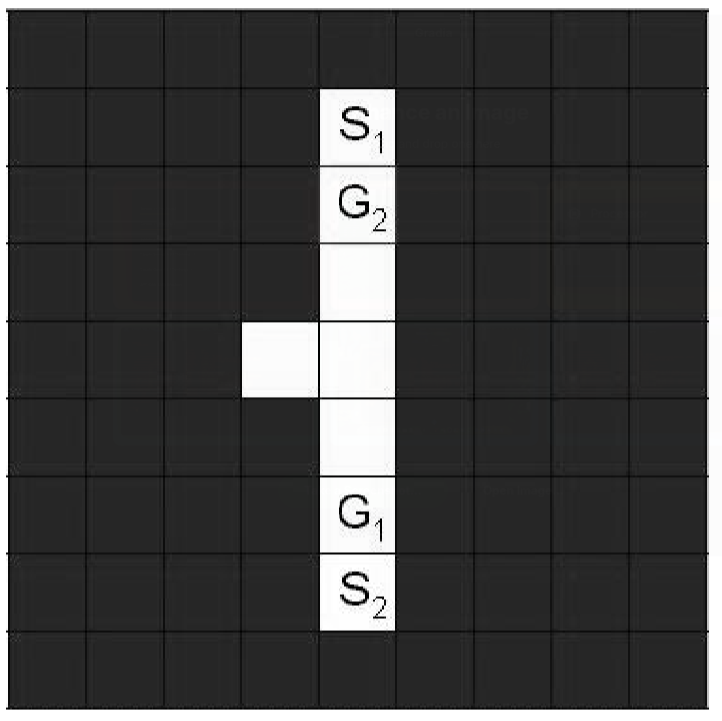
\includegraphics[width=0.5\linewidth]{img/corridor-deadlock.png}
    \captionsetup{width=0.6\linewidth, justification=justified} % Görsel genişliğinin %80'ine sığdırır ve iki yana yaslar
    \caption{Bu basit problem CA* ile çözülememektedir. \protect\ Bir etken S1'den G1'e yol alması gerekirken  diğeri \protect\ S2'den G2'ye hareket etmeye çalışmaktadır. \citep{SILVERCooperative2005}}
    \label{fig:literatür-corridor-deadlock}
\end{figure}

Bu çalışmada, tek şeritli yol yapısının getirdiği kısıtlar doğrultusunda klasik CA* algoritması üzerinde dört aşamalı, özgün bir melez (kural ve öncelik tabanlı) değişiklikler gerçeklenmiştir:

\begin{itemize}
    \item \textbf{Çizelgeleme ve Gecikmeli Çıkış Mekanizması:} Klasik algoritmalardaki rastgele veya statik sıralama yerine; araçların özel öncelik durumunu ($1-v_i$), yolun ilerisindeki araçların trafiği önce boşaltması amacıyla başlangıç konumunu ($-x_{\text{başlangıç}, i}$), hedefe kalan mesafelerini ($d_i$) ve toplam görev yüklerini ($-W_i$) kapsayan dört bileşenli bir sözlüksel öncelik vektörü $\rho_i = (1-v_i, -x_{\text{başlangıç}, i}, d_i, -W_i)$ (\autoref{sec:önceliklendirme-ve-kilitlenme-çözümü}) tanımlanmıştır. Ayrıca, uzay-zaman matrisinin yoğunluğundan kaynaklanan yapay kilitlenmeleri (artificial deadlock) engellemek adına, geçerli rota bulamayan araçların sisteme giriş anı ($t_{\text{başlangıç}}$) dinamik olarak ötelenmiştir (Delayed Release). Bu sayede sisteme araç enjeksiyonu optimize edilmiştir.
    \item \textbf{Yolda Bekleme Yasağı:} Olası fiziksel zıt yön çatışmalarını engellemek adına, araçların ana transit yol üzerinde durarak bekleme yapması (\textit{wait action}) tamamen yasaklanmıştır. Tüm durma ve yol verme eylemleri, kapasite kısıtlı cepler ($C$) ve ara depolar ($G$) ile sınırlandırılmıştır (\autoref{sec:sistem-kısıtları}).
    \item \textbf{Asimetrik Maliyet Fonksiyonu:} Algoritmanın araçları rotayı uzatan gereksiz çık-dön (\textit{yo-yo}) manevralarından kaçındırması adına asimetrik bir maliyet yapısı kurgulanmıştır (\autoref{sec:maliyet-fonksiyonu}). Hareket eyleminin maliyeti $1.0$ olarak belirlenirken, güvenli alanlarda (cep, depo, başlangıç) bekleme maliyeti $0.9$ olarak atanmıştır. Bu ağırlıklandırma, araçların ana yolu işgal etmek yerine matematiksel olarak güvenli noktalarda duraklamasını teşvik etmektedir.
    \item \textbf{Araç İçi Görev Sıralaması (SJF):} Çoklu depo ziyareti gerçekleştirecek araçların kendi içindeki görev rotaları, En Kısa İş İlk (\textit{Shortest Job First}) yaklaşımıyla optimize edilmiştir (\autoref{sec:araç-içi-görev-sıralaması}). Depolar başlangıç noktasına olan mutlak uzaklıklarına göre yakından uzağa sıralanarak, kısa mesafeli görevlerin hızla bitirilmesi, ana yolun erken boşaltılması ve uzay-zaman matrisindeki rezervasyon çakışmalarının minimize edilmesi sağlanmıştır.
\end{itemize}

Önerilen bu dinamik çizelgeleme, asimetrik maliyet yönetimi ve alana özgü kısıt tümleştirmesi, MAPF literatüründeki dar koridor kilitlenmesi problemini bu projenin kısıtları dahilinde deterministik ve düşük bir hesaplama maliyetiyle çözüme kavuşturmuştur.


    \section{Yöntem}

[Bu bölümde araştırma deseni, veri toplama araçları, ölçekler, analiz adımları ve uygulama süreci açıklanmalıdır. Şablon dosyasındaki nota uygun olarak matematiksel model, gerekli yaklaşım ve örnek uygulama burada verilebilir.]

Bu çalışma kapsamında, tek şeritli bir yol üzerinde hareket eden otonom araçların güvenli ve verimli bir şekilde yönlendirilmesi için bir çizge yapısı üzerinde uzay-zaman  tabanlı bir rezervasyon modeli kurgulanmıştır. Problem, otonom araçların belirli depo noktalarından yük alıp başlangıca dönmesini hedeflerken; çarpışma, kilitlenme ve kapasite kısıtlarını aşmamayı amaçlayan bir çizelgeleme problemi olarak ele alınmıştır.

    \begin{figure}[h!]
    \centering
    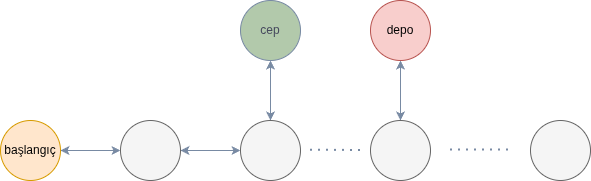
\includegraphics[width=0.7\linewidth]{img/graf-000.png}
    \caption{Genel Çizge Yapısı}
    \end{figure}

\subsection{Matematiksel Model}

Sistemin davranışını ve sınırlarını belirleyen matematiksel model; kümeler, karar değişkenleri ve kısıtlar üzerinden aşağıdaki şekilde tanımlanmıştır.

\subsubsection{Kümeler ve Parametreler} \label{sec:kümeler-ve-parametreler}

Yol uzunluğu $L = 240$ metredir.

\begin{itemize}
    \item $V = \{0, 10, 20, \dots, 240\}$: 10 metrelik adımlarla tanımlanmış yol düğümleri
    \item $C = \{80, 200\}$: Araçların bekleyebileceği cep düğümleri
    \item $G = \{70, 120, 240\}$: Araçların yük alabileceği depo düğümleri
    \item $S = \{0,40,80,120,160,200,240\}$: Her 40 metrede bir sensör bulunmaktadır.
    \item $A = \{1, 2, \dots, N\}$: Sistemdeki otonom araçlar ($3 \le N \le 20$)
    \item $T = \{0, 1, 2, \dots\}$: Ayrık zaman adımları
\end{itemize}

\subsubsection{Karar Değişkenleri}

t $\equiv$ zaman adımları olmak üzere $\forall t \in T$ olmaktadır. $x_i(t) \in V$: $i$-aracının $t$-anındaki konumunu ifade eder. $y_i$, $i$-aracının tüm görevlerini tamamlayıp başlangıç noktasına (0. metre) döndüğü anı temsil eder.

\subsubsection{Amaç Fonksiyonu (Makespan Minimizasyonu)}

Tüm araçların görevlerini tamamladığı toplam süreyi minimize etmek hedeflenmektedir:

\begin{equation}
    \min \max_{i \in A} y_i
\end{equation}

\subsubsection{Sistem Kısıtları} \label{sec:sistem-kısıtları}

\paragraph{Hareket Denklemi} Araçlar her adımda en fazla bir düğüm ilerleyebilir veya bekleyebilir.

\begin{equation}
    x_i(t+1) = x_i(t) + \Delta x, \quad \Delta x \in \{-10, 0, 10\}
\end{equation}

\paragraph{Güvenlik Mesafesi Kısıtı} İki araç arasındaki mesafe her zaman güvenli sınırlar içinde kalmalıdır. \textit{Bu kural cepler ve depolar dışındaki ana yolda mutlak geçerlidir.}

\begin{equation}
    \forall i \neq j, \forall t: |x_i(t) - x_j(t)| \ge d_{\text{min}} = 20 \text{ m}
\end{equation}
 
\paragraph{Kapasite Kısıtı} Herhangi bir $t$-anında bir cepte en fazla 1 araç, bir ara depoda ise en fazla 3 araç bulunabilir.

Bir diğer ifadeyle $\forall t$ için, $x \in C$ konumundaki araç sayısı $\le 1$. $x \in G$ araç sayısı $\le 3$ olmalıdır dolayısıyla:

Cepler için:

\begin{equation}
    \sum_{i \in A} \mathbf{1}(x_i(t) = c) \le 1, \quad \forall c \in C, \forall t \in T
\end{equation}

Depolar için:

\begin{equation}
    \sum_{i \in A} \mathbf{1}(x_i(t) = g) \le 3, \quad \forall g \in G, \forall t \in T
\end{equation}

biçiminde ifade edilebilir.

$\mathbf{1}(x_i(t) = c)$: Gösterme (Indicator) fonksiyonudur. Eğer araç o an $c$ konumundaysa $1$, değilse $0$ değerini alır.
 
\paragraph{Görev Kısıtı} Her araç, turunu tamamlamadan önce en az bir depoyu ziyaret etmelidir. Her araç turunu tamamladığında ($t = y_i$ anında), konumu $x_i(y_i) = 0$ olmalı ve $t < y_i$ için en az bir kez $x_i(t) \in G$ sağlanmalıdır.

\begin{equation}
    \exists t < y_i \text{ öyle ki } x_i(t) \in G \text{ ve } x_i(y_i) = 0
\end{equation}

\paragraph{Bekleme Eylemi Kısıtı} Bekleme eylemi yani herhangi bir aracın konumunu bir sonraki $t+1$ adımında değiştirmemesi ($x_i(t+1) = x_i(t)$), ancak bulunduğu konumun cepler ($C$), depolar ($G$) veya başlangıç ($0$) kümesinde olmasıyla mümkündür.

\begin{equation}
    (x_i(t+1) = x_i(t)) \implies x_i(t) \in C \cup G \cup \{0\}
\end{equation}

%%%%%%%%%%%%%%%%%%%%%%%%%%%

\subsection{Veri Yapıları ve Temsil}

Algoritmanın karmaşık kısıtlar altında çözüm üretebilmesi için yol ağı, araçlar ve zaman boyutu belirli veri yapıları kullanılarak soyutlanmıştır. Bu temsiller, A* algoritmasının durum uzayını verimli bir şekilde taramasına olanak tanır.

\subsubsection{Düğüm ve Çizge Yapısı}

Sistemdeki her bir fiziksel nokta, \texttt{(konum\_id, tür)} şeklinde bir üçlü demet olarak temsil edilir. Burada \texttt{konum\_id} aracın yol üzerindeki metresini (0-240), \texttt{tür} ise bulunduğu alanın fonksiyonunu (\texttt{yol}, \texttt{cep}, \texttt{depo}, \texttt{başlangıç}) belirtir. Bu ikili gösterim sayesinde, aynı koordinatta bulunan ancak farklı kapasite ve kurallara sahip olan \textit{ana yol} ve \textit{cep} düğümleri birbirinden ayrıştırılır. Çizge üzerindeki komşuluk ilişkileri, ana yol düğümlerinin birbirine doğrusal ($\pm$ 10m) bağlanması ve işlevsel düğümlerin (cep/depo) sadece kendi konumlarındaki yol düğümüne bağlanmasıyla kurulur.

\begin{figure}[h!]
    \centering
        \fbox{\rule{0pt}{4cm}\rule{0.7\linewidth}{0pt}}
%    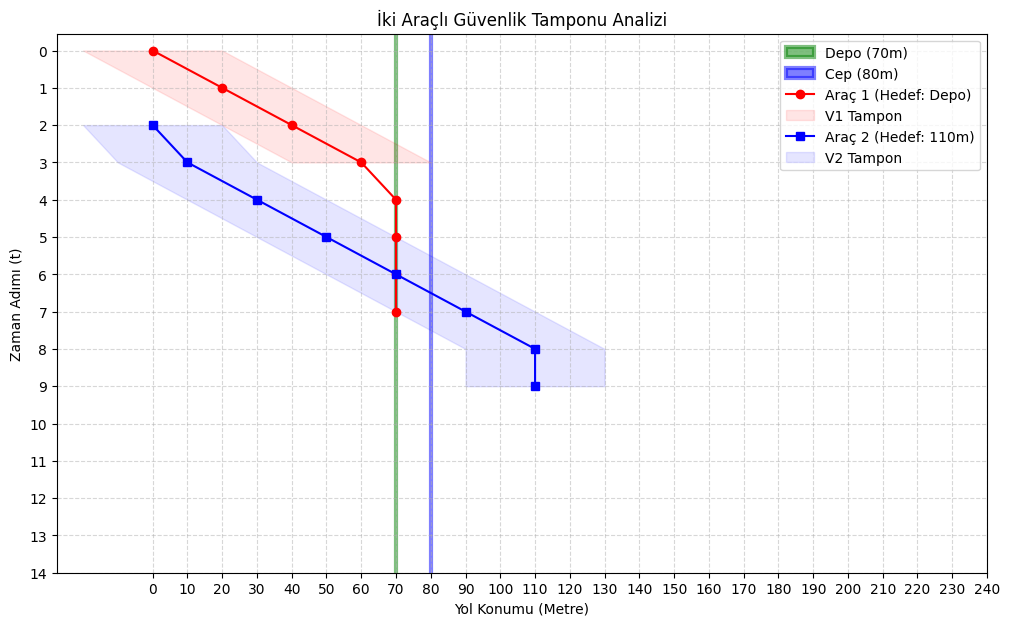
\includegraphics[width=0.9\linewidth]{img/uzay-zaman-grafiği-1.png}
    \caption{Çizge Yapısı Şekil Eklenecek}
    \label{fig:çizge-yapısı}
\end{figure}

Örneğin \texttt{(70, 'depo')} düğümü sadece \texttt{(70, 'yol')} düğümüne bağlı olurken \texttt{(70, 'yol')} düğümü \texttt{(60, 'yol')}, \texttt{(70, 'depo')} ve \texttt{(80, 'yol')} düğümlerine bağlı olacaktır. Aynı durum cep düğümleri için de geçerlidir.

Düğümler arası bağlantıları (Kenar Kümesi - $E$) veya komşuluk fonksiyonunu ($N(v)$) tanımlayabiliriz. Bir $(x, \tau)$ düğümünün komşuluk fonksiyonu $N(x, \tau)$ şu şekilde formüle edilebilir:

Ana yol düğümlerinin komşuları (hem yolda ileri/geri, hem de varsa bulunduğu konumdaki cep/depoya giriş):

\begin{equation}
    N(x, \text{'yol'}) = \{ (x \pm 10, \text{'yol'}) \} \cup \{ (x, \tau) \mid (x \in C \land \tau = \text{'cep'}) \lor (x \in G \land \tau = \text{'depo'}) \}
\end{equation}

Cep veya depo düğümlerinin komşuları (kendi içinde bekleme veya yola çıkma):

\begin{equation}
    N(x, \tau) = \{ (x, \tau), (x, \text{'yol'}) \} \quad \tau \in \{\text{'cep'}, \text{'depo'}\}
\end{equation}

\subsubsection{Durum Uzayı (State Space) Tanımı}

A* arama algoritması, sistemi statik bir harita yerine Zaman-Genişletilmiş Ağ (\textit{Time-Expanded Network}) üzerinde değerlendirir. Arama uzayındaki her bir durum, \texttt{(düğüm, zaman)} sıralı ikilisiyle tanımlanır. Bu yapı, aracın bir düğümde \textit{bekleme} eylemi yapmasını, zaman ($t \to t+1$) ilerlerken düğüm bilgisinin sabit kalması biçiminde modellemeyi sağlar. Arama, aracın başlangıç noktasındaki durumundan başlar ve hedef düğümün herhangi bir $t$-anındaki durumuna ulaşıldığında parça (\textit{segment}) bazlı olarak tamamlanır.

% Eleştiri: Zaman-Genişletilmiş Ağ (Time-Expanded Network) kavramı metinde çok iyi anlatılmış ama görseli yok. Sadece metinle 3B arama uzayını anlatmak okuyucuyu yorabilir.
% Öneri: Zamanın ($t$) dikey eksende, yol konumlarının yatay eksende olduğu, bir aracın "bekleme" eylemi yaptığında dikeyde nasıl sabit ilerlediğini gösteren basit bir Uzay-Zaman Grafiği çizip rapora eklemen, modelin anlaşılabilirliğini zirveye taşıyacaktır.

\begin{figure}[h!]
    \centering
%    \fbox{\rule{0pt}{4cm}\rule{0.7\linewidth}{0pt}}
    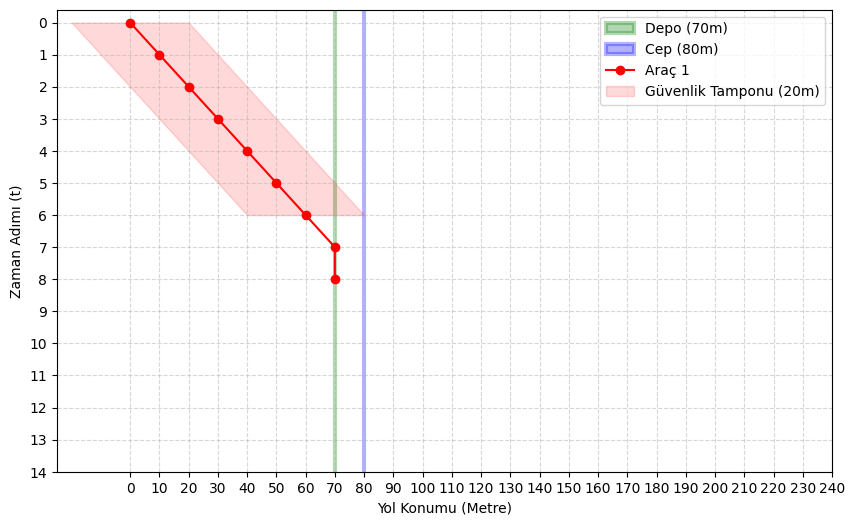
\includegraphics[width=0.9\linewidth]{img/uzay-zaman-grafiği-0.png}
    \caption{Güvenlik Tamponu ve Uzay-Zaman Grafiği}
    \label{fig:uzay-zaman-0}
\end{figure}


A* algoritmasının arama uzayı ($S$), fiziksel düğümler kümesi ($V$) ile zaman adımları kümesinin ($T$) Kartezyen çarpımıdır. Düğüm kümesi $V$ ise konumlar ($X$) ve tür ($\Gamma$) uzayının çarpımıdır.

\begin{equation}
    S = V \times T = \{ (x, \tau, t) \mid x \in X, \tau \in \Gamma, t \in T \}
\end{equation}

Burada $X = \{0, 10, \dots, 240\}$ ve $\Gamma = \{\text{yol, cep, depo, başlangıç}\}$ olarak düşünülebilir.

\autoref{fig:uzay-zaman-0}'deki senaryoda araç $x = 0$ ve $t = 0$ konumundan başlayarak sabit hızla $x=70$ konumundaki depoya ulaşmaktadır. Depoya girdiği andan itibaren güvenlik tamponu tahsisi kalkmaktadır.


\subsubsection{Merkezi Rezervasyon Tablosu ve Güvenlik Tamponu}

Araçlar arası çarpışmaları ve güvenlik mesafesi ihlallerini önlemek için merkezi bir rezervasyon veri yapısı kullanılmıştır. Bu yapı, \texttt{(konum, tür, zaman)} anahtarlarını karşılık gelen doluluk bilgisiyle eşleştiren bir sözlük (dictionary/hash map) olarak kurgulanmıştır. Bir araç için rota kesinleştiğinde, rotadaki her bir adım tabloya işlenir. Güvenlik mesafesi ($d_{min} = 20$) kuralını sağlamak adına, bir araç $t$-anında $x$-konumunda bulunuyorsa, tablodaki $x-20$, $x-10$, $x$, $x+10$, $x+20$ noktaları o zaman dilimi için rezerve edilerek diğer araçların bu bölgeye girmesi engellenir.

$i$-aracının $t$-anında oluşturduğu güvenlik tamponunu (rezerve edilen konumlar kümesi) $B_i(t)$ olarak tanımlarsak:

\begin{equation}
    B_i(t) = \{ x_i(t) + \delta \mid \delta \in \{-20, -10, 0, 10, 20\} \}
\end{equation}

Diğer araçların ($j \neq i$) çarpışma kısıtını sağlaması için rezervasyon tablosu gereği bu kümenin elemanı olmaması gerekir.


\begin{equation}
    x_j(t) \notin B_i(t), \quad \forall j \neq i
\end{equation}

\begin{figure}[h!]
    \centering
    %    \fbox{\rule{0pt}{4cm}\rule{0.7\linewidth}{0pt}}
    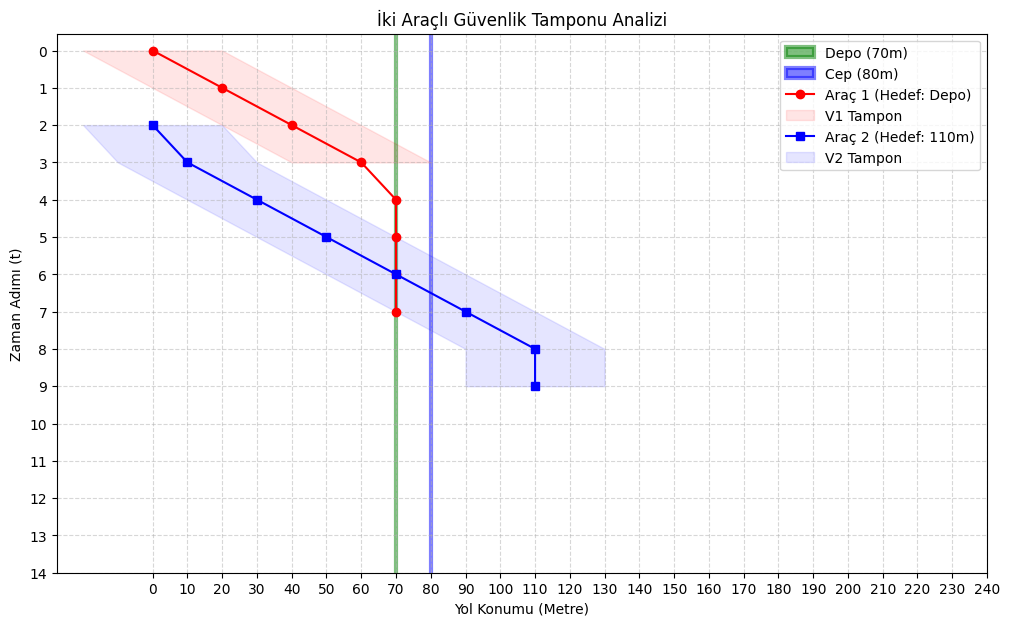
\includegraphics[width=0.9\linewidth]{img/uzay-zaman-grafiği-1.png}
    \caption{Güvenlik Tamponu ve Uzay-Zaman Grafiği}
    \label{fig:uzay-zaman-1}
\end{figure}

\autoref{fig:uzay-zaman-1}'deki senaryoda ilk araç $(0,0)$ konumundaki hareketi sonrasında $(70,t)$ konumundaki depoya ulaşmaktadır. İkinci araç ise güvenlik mesafesini koruyarak aracı takip ederek ilerelemektedir. Dikkat edilirse ilk araç depoya girdiğine güvenlik tamponu oluşmamaktadır. Öte yandan ikinci araç ise deponun konumundan geçerken güvenlik tamponu tahsis etmeye devam etmektedir. Bunun nedeni aracın depoya girmemesidir.

\subsubsection{Araç ve Görev Yönetimi}

Araçlar, kimlik bilgileri, öncelik durumları ve sıralı görev dizelgelerini içeren nesneler olarak tanımlanmıştır. Görevlerin parçalı yapısı (örneğin: 0 $\to$ \texttt{D70} $\to$ 0 $\to$ \texttt{D240} $\to$ 0), toplam yolculuğun segmentlere bölünmesini ve her segmentin bir önceki bitiş zamanını başlangıç kabul ederek ardışık olarak planlanmasını sağlar.

Bir $i$-aracının tüm görev rotasını ($M_i$), başlangıç noktasından (0) başlayıp aralarda $G$ kümesindeki depolara uğradığı ve sonunda yine başlangıca döndüğü sıralı n-demeti (ya da dizi) olarak ifade edebiliriz:

\begin{equation}
    M_i = \langle 0, g_{i,1}, 0, g_{i,2}, 0, \dots, g_{i,k}, 0 \rangle
\end{equation}

\begin{equation}
    \text{öyle ki } g_{i,m} \in G, \quad \forall m \in \{1, 2, \dots, k\}
\end{equation}

%%%%%%%%%%%%%%%%%%%%%%%%%%%%%%%%%

\subsection{Algoritma ve Çizelgeleme Yöntemi}

Problem, İşbirlikçi A* (\textit{Cooperative A*}) algoritması kullanılarak merkezi bir rezervasyon tablosu üzerinden çözülmektedir. Bu strateji, araçların birbirlerinin gelecek rotalarını bilerek hareket etmesini sağlar.

\subsubsection{Uzay-Zaman Rezervasyonu ve A* Taraması}

Her araç için rota planlaması yapılırken, 3 boyutlu bir durum uzayı (Konum $\times$ Tip $\times$ Zaman) taranır. Algoritma bir rota bulduğunda, bu rotadaki tüm konumları ve güvenlik tamponlarını (20m mesafe kuralı gereği komşu düğümleri) merkezi rezervasyon tablosuna işler. Böylece sonraki araçlar, planlarını yaparken önceden rezerve edilmiş bu alanlardan kaçınır.

\subsubsection{Maliyet Fonksiyonu} \label{sec:maliyet-fonksiyonu}

Algoritmanın araçları gereksiz manevralardan (\textit{yo-yo hareketi}) kaçındırması için asimetrik bir maliyet yapısı uygulanmıştır:

\begin{equation}
    c(s_t, s_{t+1}) = \begin{cases} 1.0, & \text{Eğer araç hareket ediyorsa} \\ 0.9, & \text{Eğer araç güvenli noktada (cep/depo/başlangıç) bekliyorsa} \end{cases}
\end{equation}

Bu düşük bekleme maliyeti, aracın yolu meşgul etmek yerine güvenli bir noktada durmasını teşvik eder. Böylece algoritma, hedefe yaklaşamayıp yolu uzatan çık-dön (\textit{yo-yo}) manevralarını $1.0 + 1.0 = 2.0$ maliyetle değerlendirirken, güvenli bir cepte/başlangıçta 2 birim beklemeyi $0.9 + 0.9 = 1.8$ maliyetle daha kârlı bulur ve gereksiz güzergahlar önlenir.

Maliyet fonksiyonu $c(s_t, s_{t+1})$, A* algoritmasının değerlendirme fonksiyonu olan $f(s) = g(s) + h(s)$ içerisinde başlangıçtan o anki duruma kadar olan kesin maliyeti ($g(s)$) hesaplamak için kullanılır:

\begin{equation}
    g(s_{t+1}) = g(s_t) + c(s_t, s_{t+1})
\end{equation}

Ayrıca algoritmanın hedef düğüme kalan tahmini mesafeyi hesapladığı sezgisel fonksiyon ($h(s)$), 1 boyutlu ağ üzerinde adım sayısı cinsinden \textit{Manhattan mesafesi} olarak tanımlanmıştır. Adım büyüklüğü $\Delta x = 10$ m olmak üzere:

\begin{equation}
    h(s_t) = \frac{|x(s_t) - x_{hedef}|}{\Delta x}
\end{equation}


\subsubsection{Araç İçi Görev Sıralaması (\textit{Local Task Sorting})} \label{sec:araç-içi-görev-sıralaması}

Algoritmanın genel performansını ve kilitlenme ihtimalini doğrudan etkileyen faktörlerden biri, her bir aracın kendi içindeki görevleri (ziyaret edeceği depoları) hangi sırayla gerçekleştirdiğidir. Bu çalışmada, araç içi görev sıralaması için En \textbf{Kısa İş İlk (\textit{Shortest Job First - SJF})} yaklaşımı kullanılmıştır. Bir araç birden fazla depoyu ziyaret edecekse, rotası başlangıç noktasına en yakın olan hedeften başlayacak şekilde sıralanır. Bu yöntemin temel amacı, araçların kısa mesafeli görevlerini hızla tamamlayıp ana yolu erken terk etmesini sağlamaktır. Ana yolun hızlı bir şekilde boşalması, diğer araçların hareket alanını genişleterek uzay-zaman tablosundaki rezervasyon çakışmalarını en aza indirir ve sistemin toplam tamamlanma süresini (\textit{makespan}) optimize eder.

Bir $i$-aracına atanmış sırasız hedef depolar kümesi $D_i \subseteq G$ olmak üzere, bu kümedeki elemanlar başlangıç noktasına (0. konum) olan mutlak uzaklıklarına göre küçükten büyüğe sıralanır. Bu işlem sonucunda $\langle g_{i,1}, g_{i,2}, \dots, g_{i,k} \rangle$ sıralı dizisi elde edilir ve sıralama kısıtı aşağıdaki eşitsizliği sağlar:

\begin{equation}
    |g_{i,1}| \le |g_{i,2}| \le \dots \le |g_{i,k}|
\end{equation}

Burada her bir $g_{i,m} \in D_i$, aracın sırayla gideceği depo konumudur. Otonom araçların her yük alımından sonra başlangıç noktasına dönme kuralı gereği, bu sıralı hedefler arasına 0. konum eklenerek aracın nihai parçalı rota dizisi ($M_i$) kurgulanır:

\begin{equation}
    M_i = \langle 0, g_{i,1}, 0, g_{i,2}, 0, \dots, g_{i,k}, 0 \rangle
\end{equation}


\subsubsection{Önceliklendirme ve Kilitlenme Çözümü} \label{sec:önceliklendirme-ve-kilitlenme-çözümü}

Sistemdeki araçlar, kilitlenmeleri (\textit{deadlock}) önlemek için belirli bir hiyerarşiye göre sırayla planlanır:

\begin{enumerate}
    \item \textbf{Özel Öncelik Durumu:} Öncelikli araçlar her zaman ilk sırada planlanır.
    \item \textbf{Fiziksel Konum Önceliği:} Tek şeritli yol hatlarında sollama imkanı olmadığından, yapay kilitlenmeleri önlemek adına hat üzerinde (0. metreden) daha ileride konumlanan araçlara öncelik verilerek öncelikle onların yolu boşaltması sağlanır.
    \item \textbf{Hedefe Yakınlık:} Mevcut hedefine daha yakın olan araçlara öncelik verilerek yolun öncelikle onlar tarafından boşaltılması sağlanır.
    \item \textbf{Gecikmeli Çıkış (\textit{Deadlock Resolver}):} Eğer bir araç için geçerli bir rota bulunamazsa, bu durum sistemin o anki yoğunluğu nedeniyle kilitlenmeye gittiğini gösterir. Çözüm olarak aracın yola çıkış zamanı ($t_{\text{başlangıç}}$) belirli bir adım kadar ötelenerek başlangıç noktasında bekletilir ve algoritma tekrar çalıştırılır. Bu mekanizma, yolda güvenli boşluklar oluşana kadar araçların sisteme girişini düzenleyerek yapay kilitlenmeleri (\textit{artificial deadlock}) engeller.
\end{enumerate}

Her $i$-aracı için çizelgeleme önceliği, üç bileşenli bir öncelik vektörü (\textit{tuple}) $\rho_i$ ile tanımlanmıştır. Algoritma bu vektörleri küçükten büyüğe değerlendirir.

Öncelik vektörünün bileşenleri şunlardır:

\begin{enumerate}
    \item $v_i \in \{0, 1\}$: Aracın özel öncelik durumu (öncelikli ise 1, değilse 0). Öncelikli araçların öne geçmesi için bu değer ters çevrilerek $(1 - v_i)$ olarak kullanılır.
    \item $-x_{\text{başlangıç}, i}$: Aracın yola çıktığı orijinal başlangıç noktası. Hat üzerinde daha ileride olan aracın küçük bir değer alarak öne geçmesi için bu değer negatif olarak eklenir.
    \item $d_i$: Aracın mevcut hedefine olan uzaklığı ($d_i = |x_{hedef} - x_i(t)|$).
    \item $W_i$: Aracın tüm görevleri boyunca kat edeceği toplam mesafe. Daha çok işi olan aracın öne geçmesi için bu değer negatif ($-W_i$) olarak vektöre eklenir.
\end{enumerate}

Buna göre $i$-aracının öncelik vektörü $\rho_i$ şu şekilde ifade edilir:

\begin{equation}
    \rho_i = (1 - v_i, -x_{\text{başlangıç}, i}, d_i, -W_i)
\end{equation}


Yalnızca hedefe olan uzaklığın ($d_i$) baz alınması, araçların farklı istasyonlara yöneldiği senaryolarda \textbf{yapay kilitlenmelere} yol açmaktadır. Örneğin; 20. ve 30. metrelerde konumlanan iki araçtan, 20. metredekinin hedefi Depo 70, 30. metredekinin hedefi ise Depo 120 olsun. Sadece hedefe yakınlık kriteri uygulandığında, 20. metredeki araç hedefine daha yakın olduğu için ($50 < 90$) ilk sırada çizelgelenmeye çalışılacaktır. Ancak tek şeritli hat üzerinde önünde bulunan 30. metredeki araç henüz hareket etmediği için $d_{\min}$ güvenlik tamponu anında ihlal edilecek ve kilitlenme oluşacaktır. Vektöre eklenen $-x_{\text{başlangıç}, i}$ bileşeni sayesinde, hat üzerinde fiziksel olarak daha önde olan (30. metredeki) araç ilk önce çizelgelenir; böylece güvenlik tamponunu arkasından gelen araç için temizleyerek yapay kilitlenmeyi engeller.

Problem kısıtları gereği, özel öncelikli araçlar daima başlangıç noktasında (0. metre) konumlanır ve tek bir görev (belirli bir depoya gidip dönme) üstlenirler. Algoritma bu araçları mutlak ilk sıraya alarak çizer. Bu kısıt, öncelikli araçların sistem henüz boşken rezerve edilmemiş bir uzay-zaman tablosunda ilerlemesini sağlar; böylece diğer araçların yaratabileceği yoğunluğa ve gecikmelere takılmadan, görevlerini matematiksel olarak mümkün olan en kısa sürede (optimal makespan ile) tamamlamaları garanti altına alınır.

İki araç karşılaştırıldığında sözlüksel sıralama (\textit{lexicographical order}) uygulanır. Eğer $\rho_i < \rho_j$ ise, $i$-aracı $j$-aracından önce çizelgelenir. Bu yapı sayesinde özel öncelikli araçlara mutlak üstünlük verilirken, eşitlik durumlarında sırasıyla hedefe yakınlık ve toplam iş yükü devreye girer.

\begin{figure}[h!]
    \centering
    %    \fbox{\rule{0pt}{4cm}\rule{0.7\linewidth}{0pt}}
    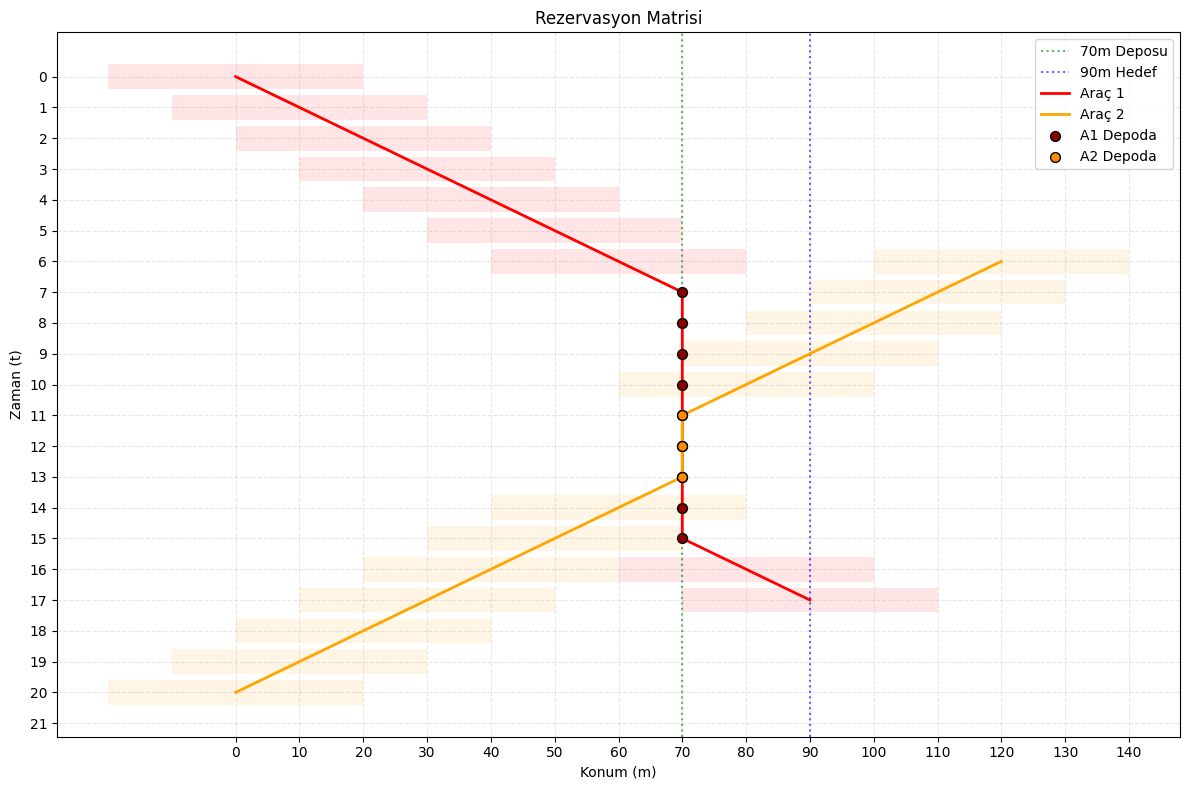
\includegraphics[width=0.9\linewidth]{img/uzay-zaman-grafiği-2.png}
    \caption{Yol Verme Senaryosu}
    \label{fig:uzay-zaman-2}
\end{figure}

\autoref{fig:uzay-zaman-2}'de daha önce çizelgelenmiş A2 aracı ve yol vermek için depoya giren A1 aracı bulunmaktadır. Bu örnekte A2 aracı depoya uğradıktan sonra depodan ayrılmakta ardından A1 aracı diğer aracın güvenlik tamponundan çıktıktan sonra depodan dışarı çıkmaktadır.

\subsubsection{Algoritma Karmaşıklığı}

% İşbirlikçi A* (CA*) algoritmasının hesaplama karmaşıklığı, arama yapılan durum uzayının (konum, tip, zaman) büyüklüğüne ve kullanılan veri yapılarına doğrudan bağlıdır. Algoritmanın performansını artıran en temel etmen, merkezi rezervasyon tablosunun bir Hash Map (sözlük) veri yapısı ile kurgulanmış olmasıdır. Bu sayede, A* algoritması yeni bir düğümü genişletirken yapması gereken $(x, \tau, t)$ durum çakışma (çarpışma ve kapasite) kontrollerini $O(1)$ sabit sürede gerçekleştirebilmektedir.

% Arama uzayının boyutu, fiziksel düğüm sayısı ($|V_{fiziksel}|$) ve algoritmanın ulaşabileceği maksimum zaman adımı ($T_{max}$) ile orantılıdır. Tek bir araç için en kötü durum zaman karmaşıklığı, 3 boyutlu graf üzerindeki standart A* davranışına paralel olarak $O(|V_{fiziksel}| \times T_{max} \log(|V_{fiziksel}| \times T_{max}))$ biçiminde ifade edilebilir. Toplam karmaşıklık ise $N$ adet araç için bu değerin araç sayısı ile çarpılmasıyla bulunur. Yoğun trafik senaryolarında, kilitlenme çözücü (\textit{deadlock resolver}) mekanizmasının devreye girmesi ve araçların yola çıkış zamanlarını ($t_{\text{başlangıç}}$) öteleyerek A* aramasını tekrar başlatması, algoritmik iş yükünü artıran (üstel büyümeye yaklaşan) bir faktördür. Ancak otonom araç yönlendirme problemlerinin doğası gereği, bu hesaplamalar araçlar yola çıkmadan önce çevrimdışı (offline) planlama aşamasında yapıldığından, elde edilen işlem süresi maliyeti sistemin kilitlenmeden güvenli çalışması adına kabul edilebilir bir düzeydedir.

İşbirlikçi A* algoritmasının zaman karmaşıklığı, fiziksel yol düğümlerinin ($V$) ve maksimum zaman adımının ($T_{max}$) oluşturduğu arama uzayına bağlıdır. Tek bir araç için en kötü durum (worst-case) zaman karmaşıklığı $O(|V| \times T_{max} \log(|V| \times T_{max}))$ olarak ifade edilebilir. Algoritmanın çalışma süresini asıl optimize eden unsur, merkezi rezervasyon tablosunun bir Hash Map (sözlük) veri yapısında kurgulanmasıdır. Bu sayede algoritmanın uzay-zaman tablosundaki çakışma ve güvenlik kontrolleri $O(1)$ sabit sürede yapılarak, dinamik araç sayısının yarattığı işlem yükü minimize edilmiştir.

        \section{Bulgular ve Senaryo Analizi}

    Senaryolardaki çizge yapısı \autoref{sec:kümeler-ve-parametreler}'de tanımlandığı gibidir. Analizlerde aksi belirtilmedikçe buradaki çizge yapılandırması kullanılacaktır.
    
    \subsection{Zıt Yön Çatışması}
    
    Bu senaryoda yazılan programın dinamik başlangıç özelliğinden yararlanarak araçların olası zıt yönde karşı karşıya gelme durumunda birbirlerine nasıl yol verdikleri analiz edilecektir.

    \subsubsection{Yapılandırma}
    
    Araçlar, görevleri ve yönleri aşağıdaki gibi yapılandırılmıştır. Araçların başlangıcı başlık 3.3.4'de verilen çizelgeleme algoritmasına göre belirlenmektedir.
    
    Araçlar $t = 0$ anında aşağıdaki konumlarda başlamaktadırlar. $A = \{1, 2, 3, 4, 5, 6 \}$ araçları için $X_{t = 0}$-konum vektörü olmak üzere:
    
    \begin{equation}
        X_{t = 0} = \{0, 0, 0, 240, 240, 240 \}
    \end{equation}
       
    \begin{itemize}
        \item $\text{Görevler} = \{ \{240\}, \{240\}, \{240\}, \{70\}, \{70\}, \{70\}\}$
        \item $\text{Yönler} = \{ 1, 1, 1, -1, -1, -1 \}$
        \item $G = \{ 70, 120, 240 \}$
        \item $C = \{ 80, 200 \}$
    \end{itemize}
    

    \begin{figure}[h!]
        \centering
        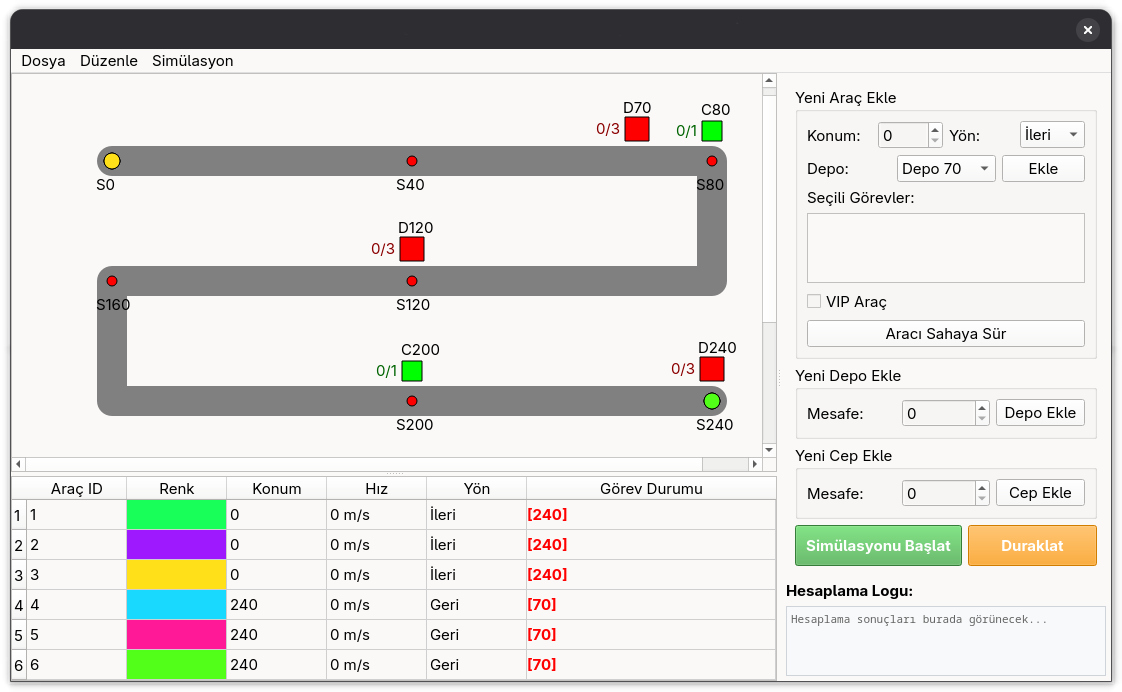
\includegraphics[width=0.7\linewidth]{img/senaryolar/0-zıt-yön-çatışması/00-başlangıç.png}
        \caption{\label{fig:zıt-yön-başlangıç}Zıt Yön Çatışması: Başlangıç Durumu}
    \end{figure}
 
    \subsubsection{Analiz}
    
    Başlangıç durumunda; (\autoref{fig:zıt-yön-başlangıç}) D240'da üç araç sola doğru yönde başlamaktadır, başlangıç konumunda ($x = 0$) ise üç araç sağ yönde başlamaktadır. Çizelgeleme algoritması gereği (\autoref{sec:önceliklendirme-ve-kilitlenme-çözümü}) önce D240'daki (A4, A5, A6) araçları önce çizelgelenmektedir. A5 ve A6 depoda beklerken A4 aracı D70'e doğru yola çıkmaktadır. Ardından güvenlik mesafesi korunarak A5 ve A6 araçları da D70 görevi için sırayla yola çıkıyorlar. Bu esnada başlangıç konumundaki A1, A2 ve A3 araçlarından A1 ve A2 yol vermek için D70 ve C80'de beklemektedirler (\autoref{fig:zıt-yön-araçların-beklemesi}).
    
    \begin{figure}[h!]
        \centering
        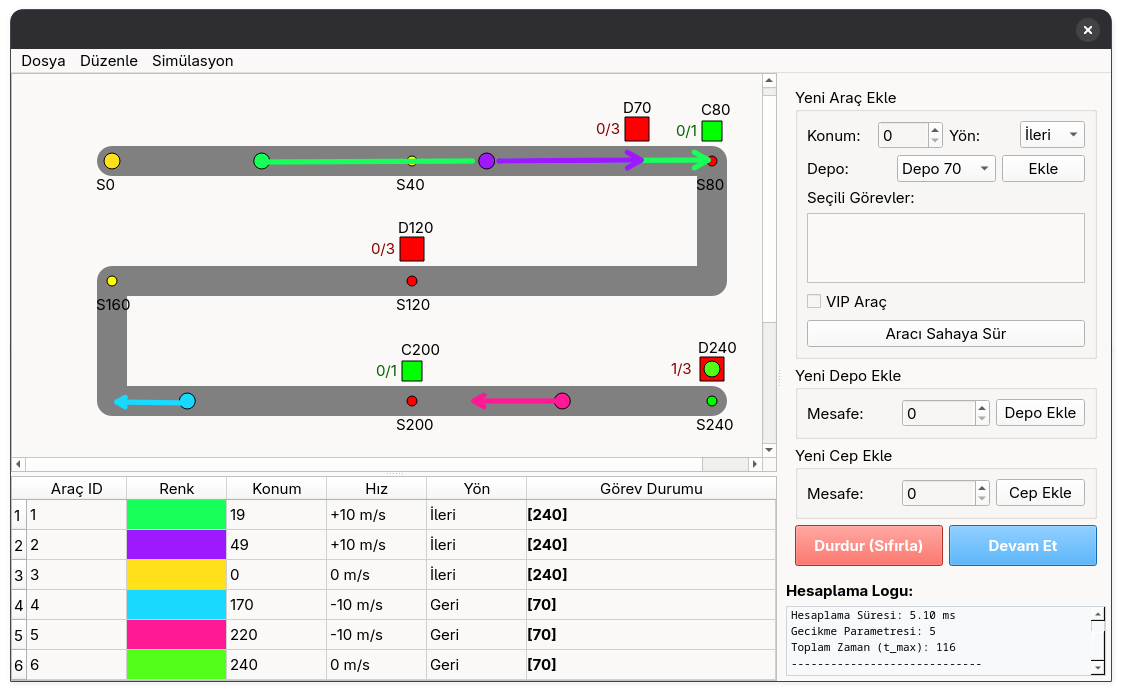
\includegraphics[width=0.7\linewidth]{img/senaryolar/0-zıt-yön-çatışması/01-ilk-iki-aracın-çıkışı (Edit).png}
        \caption{\label{fig:zıt-yön-ilk-iki-araç} İlk araçların çıkışı}
    \end{figure}
    
    A4, A5, A6 araçları D70 görevini tamamlayıp başlangıca döndükten sonra görevleri bitiyor. Ardından D70 ve C80'de bekleyen A1 ve A2 araçları sırayla D240 görevi için yola çıkmaktadırlar. Bu iki araçtan sonra A3 aracı en son yola çıkıp D120'de bu iki araca yol vermek için beklemektedir. Çizelgelemeye göre en başta olan A1 aracı yükünü alırken A2 aracı C200 cebinde bekleyip yol vermektedir. En son A3 aracı diğer araçlara yol verdikten sonra yükünü D240'dan alıp başlangıca döner (\autoref{fig:zıt-yön-son-araçların-yol-vermesi}).
    
    \begin{figure}[h]
        \centering
        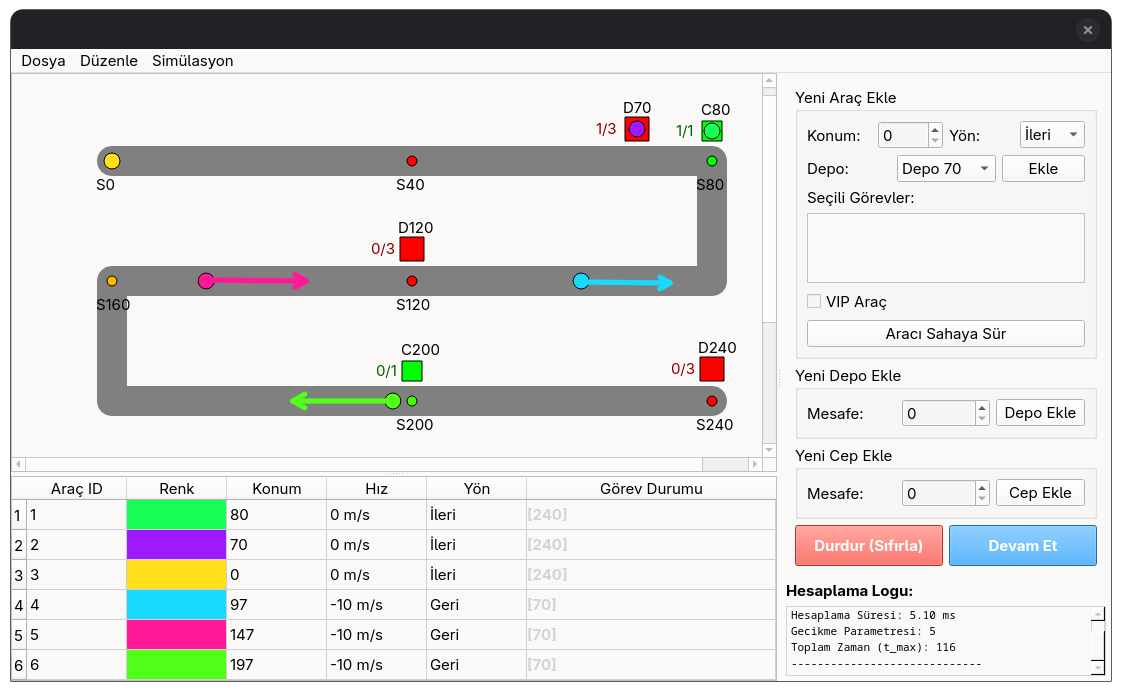
\includegraphics[width=0.7\linewidth]{img/senaryolar/0-zıt-yön-çatışması/02-araçların-beklemesi (Edit).png}
        \caption{\label{fig:zıt-yön-araçların-beklemesi} A1 ve A2 araçlarının beklemesi}
    \end{figure}
        
    \begin{figure}[h]
        \centering
        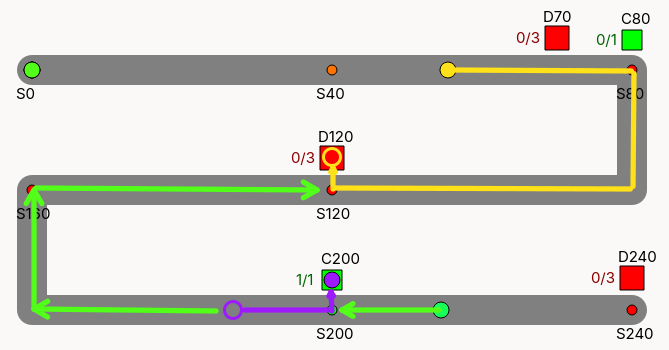
\includegraphics[width=0.7\linewidth]{img/senaryolar/0-zıt-yön-çatışması/03-son üç aracın birbirine yol vermesi (Edit).png}
        \caption{\label{fig:zıt-yön-son-araçların-yol-vermesi} A2 ve A3 aracının A1 aracına yol vermesi}
    \end{figure}
      
    \paragraph{Potansiyel Çarpışma Noktası} Kontrol mekanizması olmasaydı, zıt yönlü hareket eden $A_1$ ve $A_4$ araçları $t = 4$ anında $x = 120\text{ m}$ koordinatında kilitlenme (\textit{deadlock}) veya kafa kafaya çarpışma yaşayacaktı.
    
    \paragraph{Kilitlenme Analizi} $A_1$ aracı $C_{80}$ cebine çekilerek bekletilmiş, böylece kilitlenme olasılığı matematiksel kısıtlara uygun olarak sıfıra indirilmiştir.
    
    \subsubsection{Sonuç}
    
    Yapılan analiz sonucunda çizelgelemeye uygun olarak hareketlerine başlayan araçlar cepler ve depoları kullanarak birbirlerine yol vererek sırayla görevlerini tamamladıkları görülmüştür. Algoritmanın hesaplama süresi ve toplam zaman adımı (\textit{makespan}) \autoref{tab:zıt-yön-tablo}'da gösterilmiştir.
    
    \begin{table}[h]
        \centering
        \caption{Sonuçlar} \label{tab:zıt-yön-tablo}
        \begin{tabular}{lr}
            \hline
            Hesaplama Süresi (ms) & 5.10 \\
            \hline
            Toplam Zaman Adımı ($t_{max}$) & 116 \\
            \hline
        \end{tabular}
    \end{table}

\subsection{Darboğaz Sınaması} \label{sec:darboğaz-sınaması}
  
    Bu senaryoda araçların hepsinin tek bir depoya yoğunlaştığı durumda düzeneğin nasıl davrandığı incelenecektir. Amaca uygun olarak 10 tane araç başlangıç konumunda ve hepsinin görevi sadece D70 olacak biçimde yapılandırma yapılmıştır. Ardından sistem optimizasyonu üzerine etkisini gözlemlemek için araçların kullanabileceği bir cep sisteme eklenerek aynı senaryo tekrarlanmıştır.
    
    \subsubsection{Yapılandırma}
    
        Araçlar $t = 0$ anında aşağıdaki konumlarda başlamaktadırlar. $A = \{1, 2, 3, 4, 5, 6, 7, 8, 9, 10 \}$ araçları için $X_{t = 0}$-konum vektörü olmak üzere:
    
    \begin{equation}
        X_{t = 0} = \{0, 0, \dots, 0 \}
    \end{equation}
    
    \begin{itemize}
        \item $\text{Görevler} = \{\{70\}, \dots, \{70\}\}$
        \item $\text{Yönler} = \{ 1, \dots, 1\}$
        \item $G = \{ 70\}$
        \item $C = \emptyset $
    \end{itemize}
    
    \subsubsection{Analiz}
    
    Araçlar çizelgeleme mantığına uygun olarak kimlik numaralarına göre sırayla başlangıçtan hareket edip D70 deposuna gitmektedirler (\autoref{fig:darboğaz-başlangıç}). Bir araç yoldayken başka bir araç depoya hareket etmemektedir (\autoref{fig:darboğaz-cepsiz}). Arada bir cep olmadığından ve araçlar depoda yeteri kadar süre beklemediğinden darboğaz oluşmaktadır.
    
    \begin{figure}[h]
        \centering
        
\includegraphics[width=0.7\linewidth]{img/senaryolar/1-darboğaz/00-başlangıç.png}
        \caption{\label{fig:darboğaz-başlangıç} Darboğaz Sınaması: Başlangıç Durumu}
    \end{figure}

    Bu durumu çözmek için araya bir cep eklenebilir (\autoref{fig:darboğaz-cepli}). Cepler kümesi $C = \{ 30 \} $ olacak biçimde güncellenerek \autoref{fig:darboğaz-cepli}'deki yol yapılandırması elde edilmiştir. Cep eklendiği durumda iki araç peş peşe (güvenlik mesafesini koruyarak) çıkacaklar ve öndeki araç depodan dönüp aradaki cebi geçtikten sonra diğer cepteki araç depoya gidecektir. Cep boşaldıktan sonra ise üçüncü araç cebe girecektir. Bu durumu peş peşe çizelgelenen her araç için tekrarlanır. 
    
    Ceplerin eklenmesi durumunda araçlar hedeflerine daha yakın bir mesafeden başlayacaktır. Beklendiği üzere toplam zaman adımı ($t_{max}$) 171'den 135'e düşmüştür.
    
    \begin{figure}[h]
        \begin{subfigure}{.5\textwidth}
            \centering
            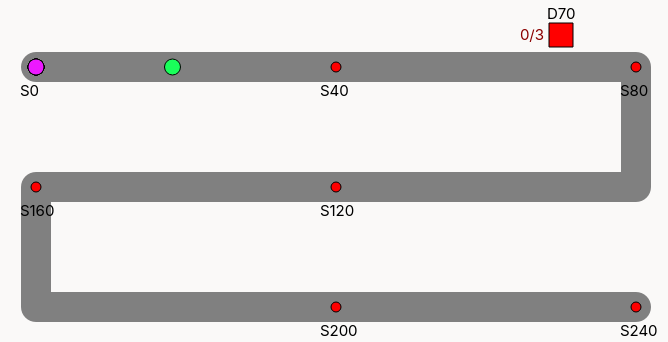
\includegraphics[width=0.9\linewidth]{img/senaryolar/1-darboğaz/01-ilk-araç.png}
            \caption{Cepsiz Durum $t_{max} = 171$}
            \label{fig:darboğaz-cepsiz}
        \end{subfigure}%
        \begin{subfigure}{.5\textwidth}
            \centering
            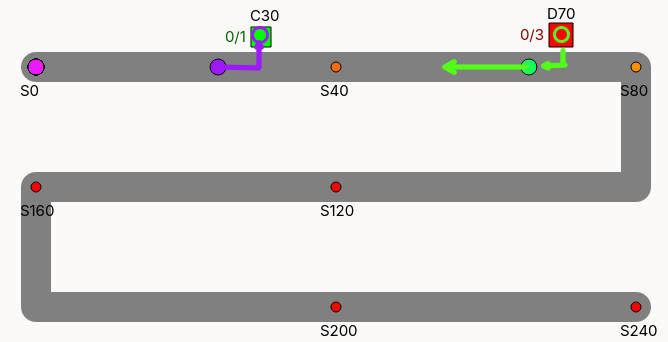
\includegraphics[width=0.9\linewidth]{img/senaryolar/1-darboğaz/02-cep-olma-durumu (Edit).png}
            \caption{Cepli Durum $t_{max} = 135$}
            \label{fig:darboğaz-cepli}
        \end{subfigure}
        \caption{Cepli ve Cepsiz Durumlarda Hareket Yönleri}
        \label{fig:darboğaz-cepli-cepsi}
    \end{figure}
    
    \subsubsection{Sonuç}

    Yapılan analiz sonucu açıkça görüldüğü üzere algoritma 10 aracın darboğaz oluşturduğu senaryoda tüm araçları başarıyla çizelgelemiş ve çarpışma durumu olmadan her aracın görevini tamamladığı gözlemlenmiştir. Darboğaz senaryosu depo ile başlangıç arasına bir cep eklenerek tekrarlandığında ise toplam zaman adımının azaldığı, hesaplama süresinin düştüğü ve araçların cepleri etkin biçimde kullanarak sistem optimizasyonunu artırdığı gözlemlenmiştir (\autoref{tab:darboğaz-tablo}).
    
    \begin{table}[h]
        \centering
        \caption{Sonuçlar} \label{tab:darboğaz-tablo}
        \begin{tabular}{l|l|l}
            Senaryo & Hesaplama Süresi [ms] & Toplam Zaman Adımı ($t_{max}$) \\
            \hline
            Cepsiz & 6.58  & 171 \\
            \hline
            Cepli & 4.43  & 135 \\
        \end{tabular}
    \end{table}

    \subsection{Stres Sınaması}\label{sec:stres-sınaması}
    
    Bu senaryoda sisteme görevleri değişen ve keyfi olarak atanmış, başlangıç noktasında konumlanan 21 araç verilmiştir (\autoref{fig:stres-görev-tablosu}). Sistemin fazla araç durumunda davranışı incelencektir. Senaryo, ceplerin ve depoların kullanımı sonucu zaman adımı değişimini ölçmek adına 21 tane sadece D240 görevine sahip araç ile tekrarlanmıştır.
        
    \begin{figure}[h]
        \centering
        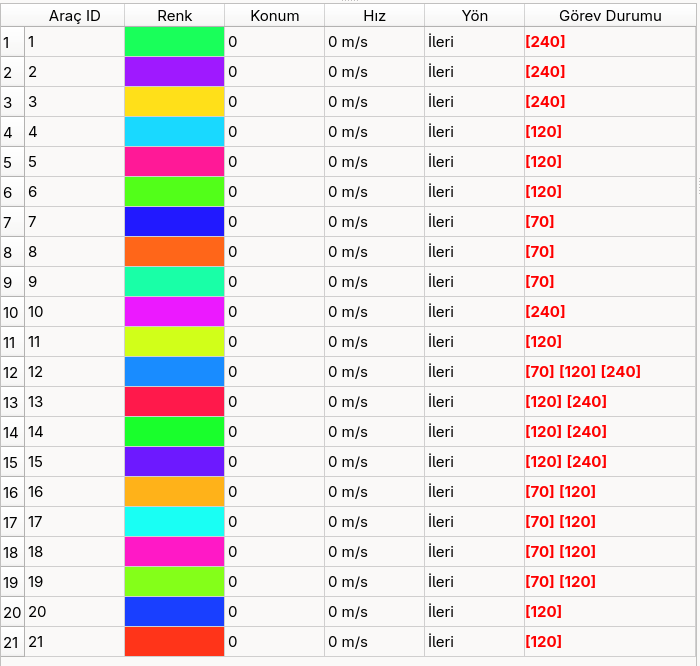
\includegraphics[width=0.7\linewidth]{img/senaryolar/2-stres/00-görev-tablosu.png}
        \caption{21 Araçlık Görev Tablosu}
        \label{fig:stres-görev-tablosu}
    \end{figure}
    
    \subsubsection{Analiz}
    
    $t_{max} = 526$ adımda ve 50.30 ms hesaplama süresiyle tüm araçlar çarpışma ve kilitlenme durumu olmadan görevlerini tamamlamıştır. Araçların görevleri boyunca cepleri ve depoları birbirlerine yol vermek için kullandıkları görülmüştür (\autoref{fig:stres-görev-anlık-görüntü}). Araçların ceplerde veya depolarda beklerken gereksiz girme çıkma durumları yerine daima bekledikleri gözlemlenmiştir.
    
    Araçların sadece D240 görevine sahip olduğu senaryodaysa (\autoref{fig:stres-tek-görev-başlangıç}) araçlar peş peşe başlangıçtan çıkmış ve sırayla uygun depo ve ceplerde önlerindeki aracın dönüşüne yol vermek için beklemeye geçmişlerdir.
    
    \begin{figure}[h]
        \begin{subfigure}{.5\textwidth}
            \centering
            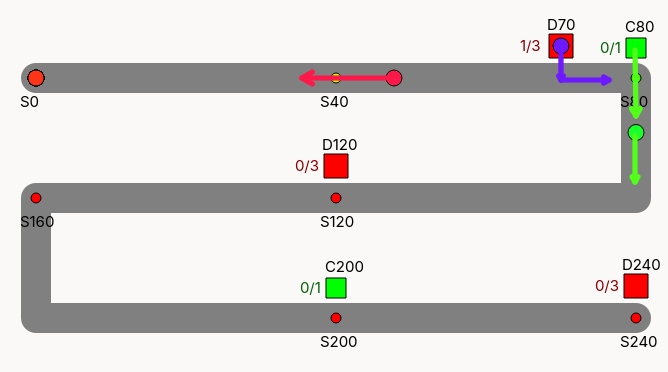
\includegraphics[width=0.9\linewidth]{img/senaryolar/2-stres/01-rastgele-bir-anda (Edit).png}
            \caption{Keyfi Görevler}
            \label{fig:stres-rastgele-bir-an}
        \end{subfigure}
        \begin{subfigure}{.5\textwidth}
            \centering
            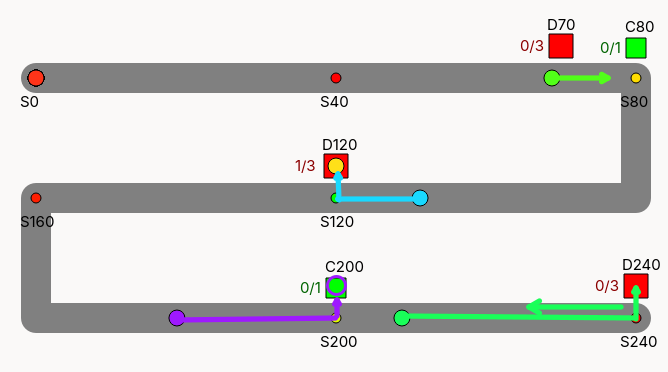
\includegraphics[width=0.9\linewidth]{img/senaryolar/2-stres/02-tek-görev-başlangıç (Edit).png}
            \caption{Tek Görev Durumu}
            \label{fig:stres-tek-görev-başlangıç}
        \end{subfigure}
        \caption{Görev Tablosu ve Sistemin Anlık Görüntüsü}
        \label{fig:stres-görev-anlık-görüntü}
    \end{figure}
    
    \subsubsection{Sonuçlar}
    
    21 araçlık senaryodaki hesaplamalar sistemde herhangi bir takılmaya neden olmadan kısa bir sürede tamamnlamıştır. Peş peşe birçok aracın \autoref{sec:darboğaz-sınaması}'de olduğu gibi aynı depoya gitmelerinden ötürü oluşan darboğaz gibi nedenlerden dolayı zaman adımının epey fazla olduğu gözlemlenmiştir.
    
    Tek görevin olduğu senaryo ile kıyaslandığında (\autoref{tab:stres-tablo}) hesaplama süresinin neredeyse 3 katına çıktığı toplam zaman adımının da 54-adım kadar düştüğü gözlemlendi. Zaman araçların başlangıçta zaman kaybetmek yerine depoda beklemesi sonucu azalsa da her t-anında yolda birçok aracın sürekli karşılaşmasından ötürü hesaplama süresi artmıştır.
    
    
    \begin{table}[h]
        \centering
        \caption{Sonuçlar} \label{tab:stres-tablo}
        \begin{tabular}{l|l|l}
            Görevler & Hesaplama Süresi [ms] & Toplam Zaman Adımı ($t_{max}$) \\
            \hline
            Değişen & 50.3  & 526 \\
            \hline
            Tek & 146.32  & 472 \\
        \end{tabular}
    \end{table}
    
    \subsection{Özel Öncelikli Araç}
    
    Bu bölümde özel öncelikli olarak belirlenen araçlara diğer araçların yol vermesi incelenecektir.
    
    \subsubsection{Yapılandırma}
    
        Araçlar $t = 0$ anında aşağıdaki konumlarda başlamaktadırlar. $A = \{1, 2, 3, 4, 5\}$ araçları için $X_{t = 0}$-konum vektörü olmak üzere:
    
    \begin{equation}
        X_{t = 0} = \{0, 0, 0, 30, 0 \}
    \end{equation}
    
    A1, A2 ve A3 araçları özel öncelikli (\textit{VIP}) araçlar olmaktadırlar. Her araç daima bu araçlara yol önceliği tanımaktadır.
    
    \begin{itemize}
        \item $\text{Görevler} = \{ \{240\}, \{120\}, \{70\}, \{70\}, \{70\} \}$
        \item $\text{Yönler} = \{ 1, 1, 1, 1, 1 \}$
        \item $G = \{ 70, 120, 240 \}$
        \item $C = \{ 80, 200 \}$
    \end{itemize}
    
    \begin{figure}[h]
        \centering
        
\includegraphics[width=0.7\linewidth]{img/senaryolar/4-vip-araç/00-başlangıç.png}
        \caption{Önceliki Araçlar: Başlangıç Durumu}
        \label{fig:vip-başlangıç}
    \end{figure}
    
    A4 aracı $(x=30, t=0)$ konumundan başlatılarak bu aracın öncelikli araçlardan önde yer alması ve öncelikli araçlara yol verme davranışının incelenmesi amaçlanmıştır. (\autoref{fig:vip-başlangıç})
    
    \subsubsection{Analiz}
    
    Başlangıçta A4 aracı D70 deposuna girdikten sonra A1, A2 ve A3 araçları $x = 70$ konumunu geçip geri dönüş yolunu boşaltana kadar depoda beklemeye devam etmektedir. Başka bir ifadeyle A4 aracı öncelikli araçlar yolu boşaltana kadar yol hakkın kendisinde olmasına rağmen depoda beklemeye devam etmektedir.
        
    \begin{figure}[h]
        \begin{subfigure}{.5\textwidth}
            \centering
            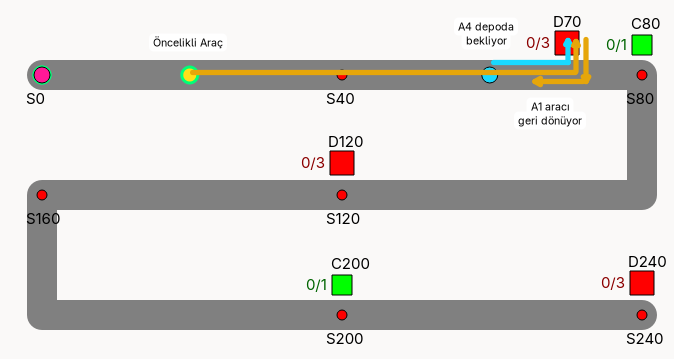
\includegraphics[width=0.9\linewidth]{img/senaryolar/4-vip-araç/01-vip-araca-yol-verme (Edit).png}
            \caption{A4 Aracı Öncelikli A1 Aracına Yol Veriyor}
            \label{fig:vip-yol-verme-0}
        \end{subfigure}
        \begin{subfigure}{.5\textwidth}
            \centering
            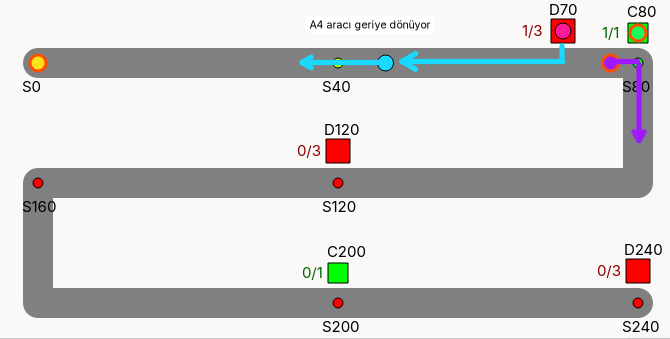
\includegraphics[width=0.9\linewidth]{img/senaryolar/4-vip-araç/02-düşük-öncelikli-en-son geri dönüyor (Edit).png}
            \caption{A4 Aracının Geri Dönüşü}
            \label{fig:vip-en-son-geri-dönme}
        \end{subfigure}
        \caption{Öncelikli Araçlara Yol Verilmesi}
        \label{fig:vip-yol-verme}
    \end{figure}
    
    \subsection{Dinamik Başlangıç}
    
    Bu senaryoda başlangıç dışında yolun ortasında başlayan araçlar ve tek bir depo kullanılarak algoritmanın dinamik başlangıçlarda kilitlenmeyi nasıl çözdüğü incelenecektir.
    
    \subsubsection{Yapılandırma}
    
    Araçlar $t = 0$ anında aşağıdaki konumlarda başlamaktadırlar. $A = \{1, 2, 3, 4, 5, 6, 7, 8, 9, 10, 11\}$ araçları için $X_{t = 0}$-konum vektörü olmak üzere:
    
    \begin{equation}
        X_{t = 0} = \{0, 0, 0, 0, 200, 240, 160, 80, 40, 60, 120 \}
    \end{equation}
    
    \begin{itemize}
        \item $\text{Görevler} = \{ \{120\}, \dots \}$
        \item $\text{Yönler} = \{ 1, 1, 1, 1, -1, \dots -1 \}$
        \item $G = \{ 120 \}$
        \item $C = \{ 60, 220 \}$
    \end{itemize}
    
    \begin{figure}[h]
        \centering
        
\includegraphics[width=0.7\linewidth]{img/senaryolar/5-dinamik-başlangıç/00-başlangıç.png}
        \caption{Dinamik Başlangıç Durumu}
        \label{fig:dinamik-başlangıç}
    \end{figure}
    
    \subsubsection{Analiz}
    
    \autoref{sec:önceliklendirme-ve-kilitlenme-çözümü}'de bahsedilen çizelgelemeye göre, önce çizelgelenen araç hedefine en yakın olan $x = 120$ konumunda başlayan A11 aracıdır. Bu aracın bulunduğu konumdaki depoya girdikten sonra doğrudan başlangıç konumuna yönelmektedir. Bu sırada yolundaki araçlardan A10 aracı bulunduğu konumdaki cebe girerken A8 ve A9 araçları ise yol verecek bir yer olmamasından ötürü başlangıç konumuna gitmektedir.
     
     \paragraph{Ceplerin Kaldırılması} C60 ve C220 ceplerinin kaldırılması durumunda ise program güvenli mesafe kuralının sağlanamaması durumundan ve rota bulunamamasından ötürü kilitlenme uyarısı vermektedir \autoref{fig:dinamik-kilitlenme-hata}.
    
    \begin{figure}[h]
        \centering
        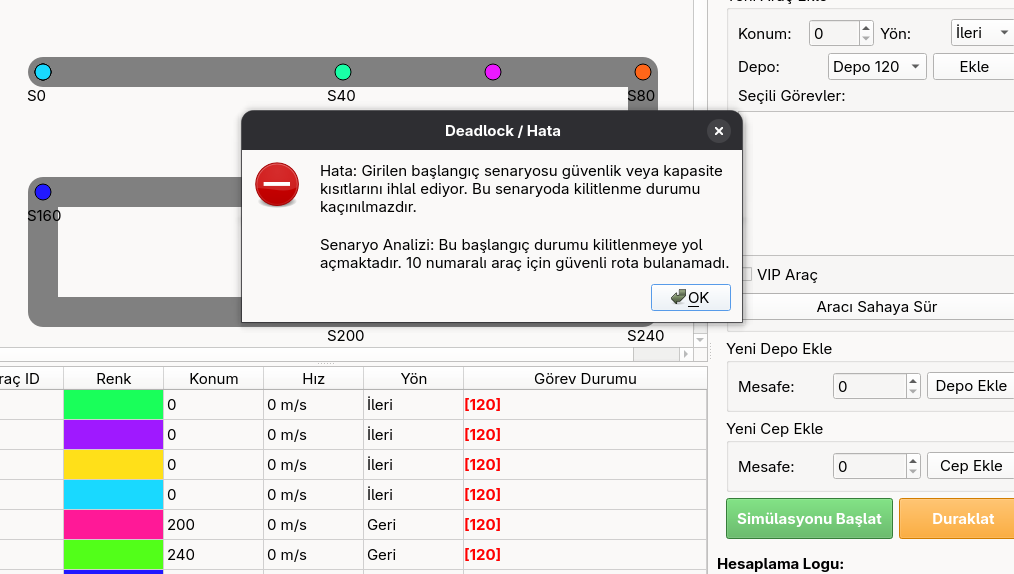
\includegraphics[width=0.7\linewidth]{img/senaryolar/5-dinamik-başlangıç/01-kilitlenme-uyarısı.png}
        \caption{Kilitlenme Uyarısı}
        \label{fig:dinamik-kilitlenme-hata}
    \end{figure}
    
    \subsection{Performans Analizi}
    
    Analizi yapılan senaryolar ardından sistem \autoref{sec:stres-sınaması}'daki tek görevli senaryo baz alınarak farklı araç sayılarındaki hesaplama performansı test edilmiştir.
    
    \begin{table}[!ht]
        \centering
        \caption{Sonuçlar} \label{tab:performans-tablo}
        \begin{tabular}{l|l|l}
            Araç Sayısı & Hesaplama Süresi (ms) & Toplam Zaman \\ \hline
            5 & 11.1 & 136 \\ \hline
            11 & 43.37 & 262 \\ \hline
            14 & 68.0 & 317 \\ \hline
            21 & 146.32 & 472 \\ \hline
            30 & 297.04 & 653 \\ \hline
            33 & 518.83 & 724 \\ \hline
            36 & 1291.78 & 779 \\ \hline
            39 & 2490.93 & 850 \\ \hline
            42 & 3854.37 & 905 \\
        \end{tabular}
    \end{table}
    
    \autoref{fig:performans-hesaplama}'de gözüktüğü üzere hesaplama zamanı araç sayısı arttıkça üstel olarak artmaktadır. Toplam görev tamamlanma zamanıysa (\autoref{fig:performans-zaman}) araç sayısına bağlı olarak doğrusal bir artış eğilimindedir.
    
    \begin{figure}[h]
        \centering
        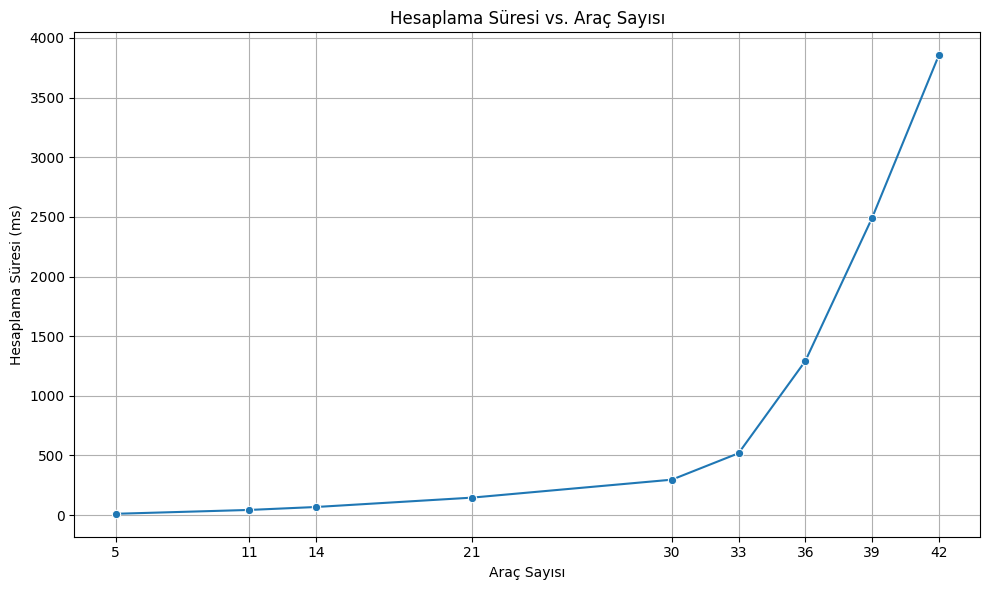
\includegraphics[width=0.9\linewidth]{img/senaryolar/3-performans/hesaplama-süresi-grafik.png}
        \caption{Hesaplama Süresi - Araç Sayısı}
        \label{fig:performans-hesaplama}
    \end{figure}
    
    \begin{figure}[h]
        \centering
        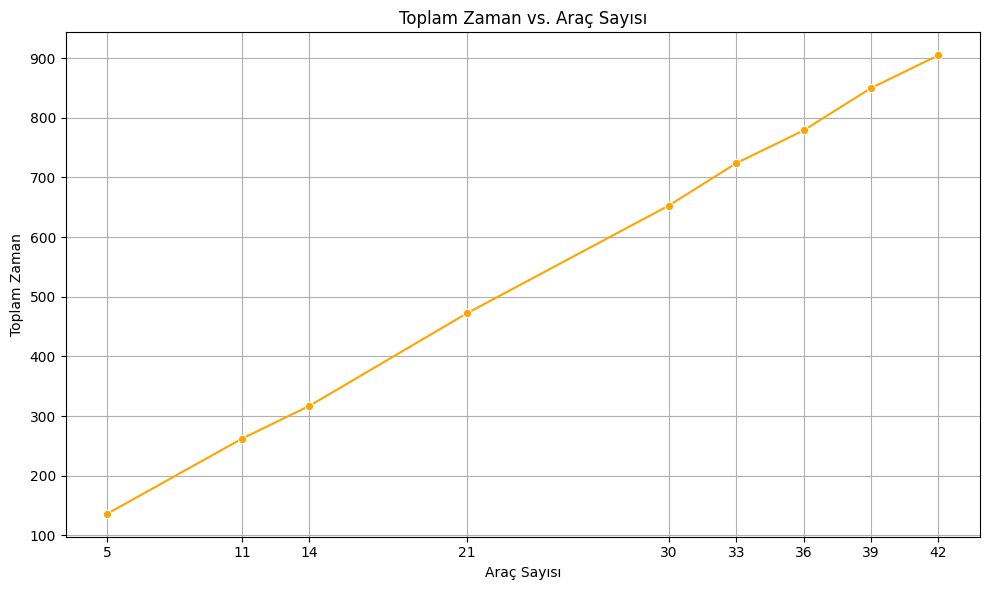
\includegraphics[width=0.9\linewidth]{img/senaryolar/3-performans/zaman-adımı-grafik.png}
        \caption{Toplam Zaman - Araç Sayısı}
        \label{fig:performans-zaman}
    \end{figure}

    
    \section{Sonuç ve Öneriler}

[Bu bölümde elde edilen sonuçlar özetlenmeli; uygulamaya ve gelecekteki çalışmalara yönelik öneriler sunulmalıdır.]

    
    \bibliographystyle{apalike}
    \bibliography{references}
    

    
\end{document}

%%%%%%%%%%%%%%%%%%%%%%%%%%%%%%%%%%%%%%%%%%%%%%%%%
%%%%%%%%%%%%%%%%%%%%%%%%%%%%%%%%%%%%%%%%%%%%%%%%%
%%%%%%%%%%%%%%%%%%%%%%%%%%%%%%%%%%%%%%%%%%%%%%%%%

    % İsteğe bağlı örnekler
\begin{table}[h!]
    \centering
    \caption{Örnek tablo başlığı}
    \begin{tabular}{ll}
        \hline
        Sütun 1 & Sütun 2 \\
        \hline
        Veri A & Veri B \\
        \hline
    \end{tabular}
\end{table}

\begin{figure}[h!]
    \centering
    \fbox{\rule{0pt}{4cm}\rule{0.7\linewidth}{0pt}}
    \caption{Örnek şekil başlığı}
\end{figure}



\begin{figure}[h]
    \begin{subfigure}{.5\textwidth}
        \centering
        \includegraphics[width=0.9\linewidth]{client-server.png}
        \caption{\label{fig:clientServer3}İstemci-Sunucu modeli üzerinde aygıtların bağlanması}
        \label{fig:sfig1}
    \end{subfigure}%
    \begin{subfigure}{.5\textwidth}
        \centering
        \includegraphics[width=0.9\linewidth]{dağıtık-sistem.png}
        \caption{\label{fig:distributed3}Dağıtık modelde aygıtların birbiri ile veri aktarımı}
        \label{fig:sfig2}
    \end{subfigure}
    \caption{İstemci-Sunucu ve Dağıtık Model}
    \label{fig:fig}
\end{figure}


%@article{ornek2024,
    %  author  = {Yılmaz, Ayşe and Demir, Mehmet},
    %  title   = {Araştırma Raporlarında Biçimsel Düzenin Önemi},
    %  journal = {Akademik Yazım Dergisi},
    %  year    = {2024},
    %  volume  = {12},
    %  number  = {2},
    %  pages   = {45--58}
    %}
%
%@book{knuth1984,
    %  author    = {Knuth, Donald E.},
    %  title     = {The {TeX}book},
    %  publisher = {Addison-Wesley},
    %  address   = {Reading, MA},
    %  year      = {1984}
    %}
%
%@inproceedings{lamport1994,
    %  author    = {Lamport, Leslie},
    %  title     = {{LaTeX}: A Document Preparation System for Technical Writing},
    %  booktitle = {Proceedings of the Technical Documentation Conference},
    %  year      = {1994},
    %  pages     = {101--110}
    %}